\documentclass[10pt,twocolumn,letterpaper]{article}
\usepackage[review,datasets]{wacv}
% Tectonic uses XeTeX; select the same Times face used by the WACV PDF build.
\usepackage{iftex}
\ifPDFTeX
  % wacv.sty already selects Times for pdfLaTeX.
\else
  \usepackage{fontspec}
  \setmainfont[
    Path=fonts/,
    Extension=.otf,
    UprightFont=NimbusRoman-Regular,
    BoldFont=NimbusRoman-Bold,
    ItalicFont=NimbusRoman-Italic,
    BoldItalicFont=NimbusRoman-BoldItalic,
    FakeStretch=1.0115
  ]{NimbusRoman-Regular}
\fi
\usepackage{float}
%
% --- color support (needed by \textcolor in \PH and \definecolor in main.tex)
%
\usepackage{xcolor}

%
% --- inline annotations
%
\newcommand{\red}[1]{{\color{red}#1}}
\newcommand{\todo}[1]{{\color{red}#1}}
\newcommand{\TODO}[1]{\textbf{\color{red}[TODO: #1]}}
% --- disable by uncommenting
% \renewcommand{\TODO}[1]{}
% \renewcommand{\todo}[1]{#1}

% --- placeholder for anything not in the evidence packet
\newcommand{\PH}[1]{\textcolor{red}{[PH:#1]}}

% --- figures live in figures/
\usepackage{graphicx}
\usepackage{subcaption}
\graphicspath{{figures/}}

% --- math macros
\usepackage{amsmath,amssymb,amsthm}
\setlength{\emergencystretch}{3em} % absorb stubborn overfull lines during page build
% Two-column article defaults to \flushbottom, which stretches sparse columns and
% opens large inter-paragraph gaps (especially around the nobreak result/proposition
% boxes). Let column bottoms be ragged instead of vertically stretched.
\raggedbottom

% The official review submission displays WACV's line numbers.

% --- framed "Result" boxes (Allen-Zhu "Physics of LM" style); pdflatex-safe
\usepackage{mdframed}
\usepackage{booktabs}  % \toprule/\midrule/\bottomrule in body curated tables
% Proxy/metric names: clean sans-serif identifier (NOT a monospace "code" look),
% hyphenated to match the figure labels, and breakable to avoid column overflow.
\newcommand{\px}[1]{\textsf{#1}}
\newcommand{\E}{\mathbb{E}}
\newcommand{\Var}{\operatorname{Var}}
\newcommand{\Corr}{\operatorname{Corr}}
\newcommand{\Phimc}{\mathcal{G}}
\DeclareMathOperator{\erank}{erank}
\newcommand{\corr}{\operatorname{corr}}
\newcommand{\partialcorr}{\operatorname{partial}}
\newcommand{\acc}{\mathrm{acc}}
\newcommand{\params}{\mathrm{params}}
\theoremstyle{plain}
\newtheorem{theorem}{Theorem}
\newtheorem{proposition}{Proposition}
\theoremstyle{definition}
\newtheorem{definition}{Definition}
% --- empirical, falsifiable regularities (NOT theorems): numbered "Result N"
% Rendered as a light-gray framed box (Allen-Zhu "Result N" register).
\theoremstyle{definition}
\newtheorem{findingthm}{Result}
\mdfdefinestyle{findingbox}{%
  backgroundcolor=black!4,
  linecolor=black!30,
  linewidth=0.4pt,
  roundcorner=2pt,
  innertopmargin=3pt,
  innerbottommargin=3pt,
  innerleftmargin=4pt,
  innerrightmargin=4pt,
  skipabove=3pt,
  skipbelow=3pt,
  nobreak=false, % allow the box to split across a column/page break, so a box that
                 % does not fit at a column bottom FILLS it and continues, instead of
                 % being bumped whole and leaving a large ragged gap below.
}
\newmdenv[style=findingbox]{findingframe}
\newenvironment{finding}[1][]%
  {\begin{findingframe}\begin{findingthm}[#1]}%
  {\end{findingthm}\end{findingframe}}
% --- inline run-in numbered "Result" environment, sharing the findingthm counter.
% Renders "\textbf{Result k (handle).} ..." inline; \cref-able as "Result k".
\newtheoremstyle{resultrunin}{4pt}{4pt}{}{}{\bfseries}{.}{ }{\thmname{#1}~\thmnumber{#2}\thmnote{ (#3)}}
\theoremstyle{resultrunin}
\newtheorem{result}[findingthm]{Result}
% cleveref names for \cref{find:...} (cleveref is loaded \AtEndPreamble in wacv.sty)
% The counter driving \cref is now `findingthm` (the inner theorem inside the box).
\AtEndPreamble{%
  \crefname{findingthm}{Result}{Results}%
  \Crefname{findingthm}{Result}{Results}%
}


% Load appendix labels while producing the separate main-paper PDF.
\usepackage{xr}
\makeatletter
\let\XRsavedbibcite\bibcite
\def\bibcite#1#2{}
\externaldocument{crossrefs/appendix}
\let\bibcite\XRsavedbibcite
\makeatother
\definecolor{wacvblue}{rgb}{0.21,0.49,0.74}
% The body and supplement are submitted as separate PDFs. Disable clickable
% links so cross-document references remain text rather than broken GoTo actions.
\usepackage[draft,pagebackref,breaklinks,colorlinks,allcolors=wacvblue]{hyperref}
\AtBeginDocument{%
  \crefname{appendix}{Sec.}{Secs.}%
  \Crefname{appendix}{Sec.}{Secs.}%
  \crefname{subappendix}{Sec.}{Secs.}%
  \Crefname{subappendix}{Sec.}{Secs.}%
}

\def\wacvPaperID{1012}
\def\confName{WACV}
\def\confYear{2027}

\begin{document}

\title{Capacity Meters That Change Sign:\\
Diagnosing Zero-Cost NAS Proxy Transport Across Search Spaces}
\author{}
\maketitle

\begin{abstract}
Zero-cost NAS proxies rank architectures from a single pass at initialization,
yet a score that ranks with accuracy in one setting can rank against it in
another. Using a 29-feature zoo on the topology and size axes of NAS-Bench-201,
we observationally separate a dominant capacity-associated factor from an
early-trainability residual. The factor explains $52.9\%/49.4\%$ of zoo
variation and remains associated with effective rank under raw/global
orientation, but the cross-axis loading cosine falls from $0.87$ under
outcome-informed orientation to $0.46$. Several raw proxies also reverse sign,
including the condition-number sum ($+0.88\,{\to}\,-0.77$); dimension and
matched-sample controls support
a dimension-linked/proxy-geometry-dependent failure, not an independent
mechanism, while matched-sample-count resampling preserves the headline reversals. Two
controlled search traps incur $+5.40$ and $+1.97$ point costs at $K{=}10$, while
two null directions incur zero. The diagnostic uses cached target-calibration
labels and is not fully label-free. These benchmark-bound results motivate
validating proxy orientation before transporting a source ranking.
\end{abstract}

\begin{figure}[t]
  \centering
  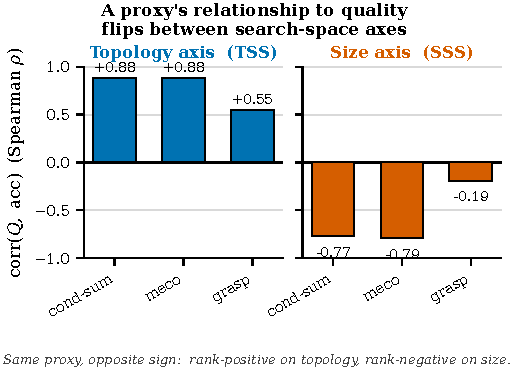
\includegraphics[width=\linewidth]{figures/fig1_signflip.pdf}
  \caption{\textbf{The cross-space sign-flip.} A proxy's rank
  correlation with quality $\corr(Q,\mathrm{acc})$ reverses sign between the
  topology axis (TSS, \emph{left}) and the size axis (SSS, \emph{right}):
  \px{cond-sum}, \px{meco}, and \px{grasp} run $+0.88,+0.88,+0.55$ on topology
  but $-0.77,-0.79,-0.19$ on size (\cref{sec:result4}).}
  \label{fig:signflip}
\end{figure}

%% (analysis-pipeline overview -- fig:overview -- relocated to the
%%  appendix Extended-results section for length; referenced via
%%  \cref{fig:overview}.)

\section{Introduction}
\label{sec:intro}

% fig:signflip is on page 1 (sec/0_abstract.tex); fig:overview is in the appendix.

Neural architecture search is bottlenecked by evaluation: training a candidate
costs GPU-days, and a search visits thousands. Zero-cost
proxies~\cite{abdelfattah2021zerocost} aim to reduce this bottleneck, ranking
an architecture from a single forward--backward pass at initialization, and on any
\emph{single} benchmark several rival a trained predictor~\cite{krishnakumar2022nbsz}.
They are often interpreted as \emph{capacity-associated} surrogates, tracking
parameters and FLOPs about as well as accuracy on some benchmarks
~\cite{ning2021evaluating,white2021powerful,kadlecova2024graf}, a proposed route
to cheap evaluation.

However, two observations about this zoo are in tension: many proxies correlate
with capacity, yet proxy quality is not reliably portable
~\cite{ning2021evaluating,white2021powerful,krishnakumar2022nbsz}. A proxy that
tops one benchmark or axis can be anti-correlated with accuracy on another. The
condition-number sum \px{cond-sum}, for example,
runs positive ($+0.88$) as wiring varies and negative ($-0.77$)
as width varies: the same published statistic, with opposite sign across axes
(\cref{fig:signflip}). We ask which statistical structures accompany this
transport failure and whether it changes a budgeted search outcome.

Rather than build a new proxy, we analyze the structure associated with existing
scores. The clean instrument is NAS-Bench-201~\cite{dong2021natsbench}:
its topology axis varies wiring at fixed width and its size axis varies width at
fixed wiring, so each axis turns \emph{one} knob, where a cross-\emph{benchmark}
comparison would confound family, dataset, and parameterization at once. Treating
a $29$-feature aligned zoo as one instrument, we organize each proxy's accuracy correlation
(\cref{eq:decomp}) into a \emph{capacity} term, computable label-free from the
representation spectrum, and a \emph{trainability residual} read against a measured
target $T$, the early-descent rate of the real training curve. Coincidentally,
NAS-Bench-Suite-Zero reports an ensemble adds up to $+42\%$ over the best single
proxy~\cite{krishnakumar2022nbsz}; we do not chase that number; we test how much
of a related complementarity gain remains after capacity adjustment
(\cref{app:access-evidence}). This decomposition is descriptive rather
than causal: it separates a dominant capacity-associated factor from an
early-trainability residual and then tests how both behave under transport.

Taken together, the evidence supports three bounded conclusions
(\cref{fig:results,fig:portability,fig:signflip}). First, both axes contain a
dominant capacity-associated factor, but outcome-informed orientation overstates
cross-axis loading-direction agreement. Second, a capacity-orthogonal
early-trainability association remains partly readable at initialization. Third,
several leading raw proxies reverse sign under transport, while other proxies---
including recent controls---remain positive on both axes. Concretely, we
contribute:
\begin{enumerate}\itemsep2pt
\item A \textbf{capacity--trainability decomposition} (\cref{eq:decomp}): a
dominant capacity-associated factor (\cref{sec:result1}, with the narrow
label-free yardstick of Proposition~\ref{thm:bound}) and a smaller,
capacity-orthogonal trainability association (\cref{sec:result2}) that is partly
init-accessible (\cref{sec:result3}).
\item An \textbf{empirical test} of a proposed ``label-free ceiling'' on these
benchmarks (\cref{sec:result5}): on the topology axis the best proxies largely close
the gap themselves, so the binding limitation there is portability, not magnitude;
on the size axis the residual increment sits at the noise floor.
\item A \textbf{tiered portability map} (\cref{sec:result4},
\cref{fig:portability}): three motivating within-NB201 examples, $9/13$
descriptive reversals across the broader map, and four strictly supported
cross-benchmark instances. Dimension controls narrow \px{cond-sum} to a
dimension-linked/proxy-geometry-dependent failure rather than an independent
mechanism.
\item A \textbf{controlled search consequence} (\cref{sec:searchtransfer}): two
named traps cost $+5.40$ and $+1.97$ points at $K{=}10$, while two null
directions cost zero. The target-calibrated screen is separated from target-EVAL
scoring but is not fully label-free, and we do not claim universal superiority.
\item A \textbf{reusable artifact design} (\cref{sec:artifact}): we construct a
cross-space portability map from per-architecture proxy values and
per-(proxy, space-pair) sign-stability annotations.
\end{enumerate}

\noindent Our study is \emph{observational}: we turn no controlled knobs and make
no causal claims; limitations, including the weaker size-axis arm ($n{=}138$
full-zoo), are detailed in \cref{sec:limitations}. The appendix supplies the
dependency layer under each result, organized as a per-conclusion dependency map
(\cref{app:map}).

\section{Related Work}
\label{sec:related}

% NOTE: the page-1 concept figure (\cref{fig:signflip}) is floated from the
% abstract (sec/0_abstract.tex); the analysis-overview figure (\cref{fig:overview})
% is in the appendix. We reference them here rather than redefining them.

The zero-cost NAS literature has largely asked \emph{how to build a proxy
that ranks better}; we instead study the statistical structure associated with
existing proxy scores, organizing
each proxy's quality correlation into a capacity term and a residual trainability
term (\cref{eq:decomp}) and studying the size, accessibility, and sign-stability of
the two (expanded in \cref{app:related-ext}).

\noindent\textbf{Capacity and expressivity proxies} score the richness an
architecture can express at init (NEAR~\cite{near2025} via effective rank,
Dextr~\cite{dextr2025} via a spectral condition number (its \px{cond-sum} we
reimplement at parity), Zen-NAS~\cite{lin2021zen} via Gaussian-perturbation
response) but none prices \emph{how much of every other proxy is largely the same
number}; \cref{sec:result1} shows a single component aligns closely with
effective rank.
\noindent\textbf{Trainability and gradient proxies} score how easily a net will
train, from one-minibatch gradient/Jacobian/NTK statistics
(ZiCo~\cite{li2023zico}, TE-NAS~\cite{chen2021tenas},
\px{jacob-cov}~\cite{jacobcov}, GradSign~\cite{gradsign},
MeCo~\cite{jiang2023meco}); what is open is whether, with capacity held fixed,
anything remains for them to read at init, which \cref{sec:result2,sec:result3}
supply as the second term of \cref{eq:decomp}.
\noindent\textbf{Ensembles and joint proxies} mix the two (AZ-NAS~\cite{aznas2024}
ensembles four axes, InTrain~\cite{intrain2026} multiplies a capacity term by a
gradient-health term, while SWAP-NAS~\cite{peng2024swap} scores sample-wise
activation patterns). Several evaluated constituents reverse between axes,
whereas SWAP and AZ-NAS remain positive on both
(\cref{sec:result4}); this mixed evidence motivates validating a recipe's
orientation rather than assuming universal transport.
L-SWAG~\cite{casarin2025lswag} is treated as uncovered rather than assigned an
approximated score because no official, licensed, auditable implementation was
available for this study.
\noindent\textbf{Benchmarks and the cross-space critique} document these effects
without a single account: rankings are inconsistent across spaces and many proxies
correlate with accuracy via parameter count~\cite{ning2021evaluating,white2021powerful},
simple features rival learned proxies~\cite{kadlecova2024graf}, and
NAS-Bench-Suite-Zero~\cite{krishnakumar2022nbsz} reports combining $13$ proxies adds
up to $+42\%$ over the best single one. We do not chase the $+42\%$ (our
same-direction gain is a conservative $+13.8\%$ (TSS) / $+1.0\%$ (SSS)) but
\emph{relate the observed gain to two associations}: a leading
capacity-associated term (\cref{sec:result1}) and a residual associated with the
external early-training target (\cref{sec:result3}); the cross-space
inconsistency is summarized by the sign reversals of
\cref{sec:result4}; against our own framing we refute a strict label-free ceiling
(\cref{sec:result5}). A measurement-provenance inventory and compute accounting
are provided in \cref{app:provenance-inventory}.
\noindent\textbf{Kernel spectral bias} we borrow only as a map: the picture of
Canatar \etal~\cite{canatar2021spectral} (and Bordelon--Pehlevan) reads a label-free
statistic's reachable target as the at-init NTK's kernel-regression error, and our
single formal statement (\cref{thm:bound}) bounds that \emph{frozen} target, not
trained accuracy. The observed proxy--trainability associations therefore do not
follow from the proposition (\cref{sec:result2,sec:result3}). The proposition is
motivation; the contribution is the empirical decomposition.

\section{Setup: One Instrument, One Knob at a Time}
\label{sec:setup}

The object of this paper is a reversal visible in \cref{fig:signflip}:
a zero-cost proxy that is among the leading predictors of accuracy on
one axis of NAS-Bench-201 becomes one of the more \emph{anti}-correlated
on the other, sign-reversed, the within-benchmark face of the field's
documented cross-benchmark inconsistency. To make that reversal a clean
measurement we hold the network family, the dataset, the proxy code, and the
accuracy table fixed and vary \emph{one} architectural knob: wiring on one axis,
width on the other. This section pins down each controlled piece and states
plainly what we do and do not claim.

\textbf{Benchmark and two axes.}
We use NAS-Bench-201~\cite{dong2020nasbench201} via
NATS-Bench~\cite{dong2021natsbench}. Its value is that it exposes \emph{two}
architectural axes over the \emph{same} dataset (CIFAR-10), each varying a single
knob. The \emph{topology axis} (TSS) varies cell wiring (which operation occupies
each of the six edges of a fixed-width cell) so architectures differ in
\emph{connectivity} at roughly constant width. The \emph{size axis} (SSS) varies
the channel width of a fixed cell topology, so architectures differ in
\emph{capacity} (parameters and nominal channel width) at fixed wiring. Studying
both is the point, not a robustness afterthought: because TSS and SSS each turn
one knob, the same statistic, the same code, on the same family and dataset, can
relate to accuracy in opposite ways depending on whether topology or width
varies (\cref{fig:signflip}, \cref{sec:result4}). A single-axis benchmark cannot
show this: the reversal needs two clean knobs that vary topology and width in
different ways. Accuracies are the CIFAR-10 test accuracies
cached in NB201 (TSS hp=200, SSS hp=90), never trained by us.

\textbf{The 29-feature aligned zoo, and sign orientation.}
We analyze \textbf{29} aligned at-init features in four groups
(\cref{tab:setup-zoo} lists every member). \emph{Standard} (12) collects
established metrics used by NAS-Bench-Suite-Zero~\cite{krishnakumar2022nbsz} (including
\px{zico}~\cite{li2023zico}, \px{meco}~\cite{jiang2023meco},
\px{zen}~\cite{lin2021zen}, and \px{ntk}~\cite{chen2021tenas}).
\emph{Spectral} (7) are functionals of the feature-map singular
spectrum: the Dextr inverse-condition-number sum \px{cond-sum} and stable sum
\px{stable-sum}~\cite{dextr2025}, and the R\'enyi-$\alpha$ effective ranks
$R_\alpha$ for $\alpha\in\{0.5,2,4,8,16\}$; $R_1$, the effective-rank
capacity anchor from NEAR~\cite{near2025}, is held out from the proxy PCA.
\emph{Label-free probes} (9, the \px{Q-*} family) comprise four NTK/Gram-spectrum
summaries (log condition, log trace, effective rank, and log largest eigenvalue),
ZiCo-style gradient variation and feature/gradient coherence under random versus
$90^\circ$/channel-rotated inputs, and a rotation-adaptivity score.
And a single \emph{label-using oracle} (1), \px{Q-zico-oracle}, consumes the real
labels: it is held apart as an upper reference, flagged (``LABEL'') wherever it
appears, and excluded from every label-free claim. This 29-feature aligned zoo is
distinct from the 13-proxy common set used for the seven-column portability map.
Proxies disagree on which direction predicts higher accuracy, so the aggregate
analysis (e.g.\ the PCA of \cref{sec:r1}) orients each proxy
\emph{within each axis} by the sign of
its Spearman correlation with accuracy, falling back to the documented prior
direction only when the data correlation is negligible (\px{plain}, $\rho=-0.01$
on TSS). Because this rule uses the outcome separately on each axis, we also
report raw and globally fixed orientation. Column-sign reflection
leaves PCA variance and score/capacity association unchanged but reduces the
cross-axis loading cosine from $0.869$ to $0.461$; we therefore do not interpret
the outcome-informed directional loading agreement as portable structure.
\label{sec:setup-orient}

\textbf{The decomposition lens.}
We read the aligned zoo one term at a time. For a proxy $Q$ the rank relationship
to accuracy is organized into a \emph{capacity-associated} part, a dominant
principal component whose scores track effective rank on both axes, and a
\emph{trainability residual}, whose per-proxy direction is tested for transport
sensitivity:
\begin{equation}
\label{eq:decomp}
\displaystyle
\underbrace{\corr(Q,\acc)}_{\text{proxy}}
\;\rightsquigarrow\;
\underbrace{\vphantom{\big|}\text{capacity}}_{\substack{\text{PC1}{\approx}\erank\\ \text{(associated)}}}
\;\rightsquigarrow\;
\underbrace{\vphantom{\big|}\text{trainability}}_{\substack{\partialcorr(Q,T\mid\mathrm{cap})\\ \text{(association)}}}.
\end{equation}
This is descriptive bookkeeping, not a numeric identity: \cref{eq:decomp} names the
two terms \cref{sec:cap-train} reads off in turn, and the formal yardstick below
prices only its capacity term.

\textbf{The trainability target $T$ (external, not a proxy).}
Separating a capacity component from a trainability component requires a
ground-truth notion of how readily an architecture trains, one that does
\emph{not} come from a proxy, or the separation collapses into a self-consistency
check. We therefore define the trainability target $T$ as the \emph{early-training
learning rate} $T_{\mathrm{slope}}$: the OLS slope of the \emph{train}-accuracy
curve over the first epochs (hp=12, epochs 0--4), read off the NATS-Bench training
curves, so larger $T$ means faster early learning. $T$ is finite on every sampled
architecture on each axis and carries a monotone relationship to accuracy in the
premise check. Because $T$ comes from training curves rather than proxies,
partialling a proxy against $T$ is a comparison against an \emph{external}
benchmark measurement, which makes the downstream residual operationally
distinct from proxy self-consistency. The three objects this study leans on (the
zero-cost proxy, the kernel picture, and $T$) are fixed in \cref{app:background}.

\textbf{Faithfulness precondition: the spectral arm is faithful.}
Before reading any cross-space behavior off the zoo, we validate our spectral
proxy implementations against the official Dextr harness. \px{cond-sum} reproduces the
inverse-condition-number statistic at parity and attains Spearman $+0.8868$ with
accuracy on TSS, consistent with the published Dextr value
$\approx0.88$~\cite{dextr2025}. The TSS parity check makes a simple
implementation mismatch less plausible, but it does not by itself validate a
causal account of the SSS behavior. The full parity check, the
hook-exception count, and the data-quality flags are in
\cref{app:faithfulness}.
\label{sec:setup-faithfulness}\label{sec:faithfulness}

\textbf{Populations and sample sizes.}
Coverage differs by proxy family, so each axis carries two principal sample sizes
(\cref{tab:setup-n}, \cref{app:pops}). The \emph{full-zoo join} intersects all
four measurement tables and contains $n=324$ TSS and $n=138$ SSS rows before
analysis-specific finite-value masks. The 29-feature PCA-complete population is
$n=317/138$; decomposition and per-proxy analyses state their own eligible
counts. The \emph{standard-proxy} population uses only the standard proxies, which
reach more architectures, $n=1000$ (TSS), $n=425$ (SSS), with effective rank and
$T$ present on the full-zoo subset. The SSS full-zoo arm ($n{=}138$) is the binding
sample-size constraint, flagged throughout as the weaker arm. Three proxies are
computed on separate single-architecture infer.tiny nets and merged in; two
(\px{nwot}, \px{epe-nas}) return a degenerate value on chance-level architectures
and are listwise-dropped, a conservative choice detailed in \cref{app:pops}.
The inclusion audit confirms that the 138 SSS records arise from the
deterministic table intersection, but also finds a mild shift toward
higher-accuracy/larger models; we retain this representativeness limitation.

\textbf{An observational study, stated up front.}
We turn no controlled architectural knob and intervene on nothing: we read
proxies, accuracies, and training curves off cached benchmark tables and
correlate them. Every number in \cref{sec:cap-train,sec:crossspace} is therefore
\emph{correlational}, and we make no causal claims. The full decomposition is
confined to NB201's TSS and SSS, the two axes where both $T$ and the spectral
arm are available, with the weaker SSS arm ($n{=}138$ full-zoo) flagged
throughout; the cross-space flip on $\corr(Q,\acc)$ we additionally confirm
generalizes across NB101, NB201, NB301, and TransNAS-Bench-101
(\cref{sec:generalize}). Read each subsequent number as a description of these
benchmarks, not as a controlled or causal finding. Full populations, the
leakage-clean cross-validation, and the bootstrap protocol are in
\cref{app:expdetails}; every body number traces to a logged source
(\cref{app:repro}).

\textbf{A formal yardstick (one knob has a ceiling).}
\label{sec:theory}\label{sec:theory-map}%
The kernel spectral-bias picture offers a narrow formal yardstick. Within that
picture the spectrum is label-free whereas the target coefficients are not; this
does not characterize every signal an at-init statistic may carry. The standard
map~\cite{canatar2021spectral,bordelon2020spectrum} (qualitative only; restated in
\cref{app:external}) has one certifiable consequence for a fixed target and
information set.

\begin{proposition}[Label-free resolution limit]
\label{thm:bound}
Fix a probability space and let $\Phimc$ be the sub-$\sigma$-algebra generated by
the label-free at-init information. For a target $Y$ with $0<\Var(Y)<\infty$,
define the \emph{frozen-kernel resolution limit}
\begin{equation}
\label{eq:r2cap}
R^2_{\mathrm{cap}}\;:=\;\frac{\Var\!\big(\E[Y\mid\Phimc]\big)}{\Var(Y)}\;\in\;[0,1].
\end{equation}
Then for any $\Phimc$-measurable statistic $S$ with $0<\Var(S)<\infty$,
\begin{equation}
\label{eq:bound}
\Corr^2(S,Y)\;\le\;R^2_{\mathrm{cap}}.
\end{equation}
\end{proposition}
\noindent\emph{Scope.}\label{sec:theory-bound}{} \cref{eq:bound} bounds the squared \emph{Pearson}
correlation (not the rank $\rho$ we report), with $Y$ read as the \emph{frozen
at-init NTK} kernel-regression error, \emph{never} trained accuracy, and
acquires content only on a \emph{restricted} information set (a finite feature
dictionary), since the full $\Phimc$ contains architecture identity and makes the
bound vacuous. Proof in \cref{app:proof}; the spectral-bias map and the longer
scope discussion are in \cref{app:external}.

\noindent
This is a label-free statistic's ruler: it bounds the \emph{frozen at-init NTK}
error, never \emph{trained accuracy} (proof \cref{app:proof}; the spectral-bias map
is \cref{app:external}).

\section{What Recurs: Capacity Association and an Accessible Trainability Residual}
\label{sec:cap-train}
\enlargethispage{-\baselineskip}

\noindent
We read the oriented $29$-proxy zoo (\cref{sec:setup}) one term of the
decomposition lens \cref{eq:decomp} at a time: summarize the zoo by PCA, treat the
leading component as an empirical \emph{capacity} axis, and ask what survives once
capacity $\{\erank,\params\}$ is held fixed against the directly measured
\emph{trainability} target $T$. A scope caveat governs everything below:
Proposition~\ref{thm:bound} prices only the capacity term of \cref{eq:decomp}, and
only for the frozen at-init NTK target, not for the trained accuracy these findings
are about (\cref{sec:setup}). Both axes are analyzed, with sample sizes stated
per analysis: the joined full-zoo cohorts contain $324/138$ rows, whereas the
29-feature PCA-complete cohorts contain $317/138$. Each result traces to a body
exhibit and corresponding appendix evidence (\cref{app:map}).

%-------------------------------------------------------------------------
% CLUSTER SUMMARY BOX (Results 1-4).
%-------------------------------------------------------------------------
\begin{findingframe}
\textbf{Associated structure in the zoo, in brief} (\cref{fig:results}). To first order the
proxy zoo contains a dominant \emph{capacity-associated factor} (PC1 scores track
effective rank and explain ${\sim}$half the variance on both axes), but a
capacity-orthogonal
early-training term ($\partialcorr{\approx}{+}0.6$) remains after capacity
adjustment and is partly predictable at initialization; the axis-specific best
label-free proxies (\px{meco} on TSS, \px{synflow} on SSS) close most of the
observed gap, so no empirical ceiling is detected on these
benchmarks.
\end{findingframe}

\noindent
We summarize above and elaborate next, in the order the findings earn.

%-------------------------------------------------------------------------
% HERO EXHIBIT: the kept 3-panel results figure (covers Results 1-4).
%-------------------------------------------------------------------------
\begin{figure*}[t]
  \centering
  {\small\bfseries
  \makebox[\linewidth][c]{%
    \parbox{0.31\linewidth}{\centering (a) PCA: dominant factor}\hfill
    \parbox{0.34\linewidth}{\centering (b) orientation-sensitive partials}\hfill
    \parbox{0.31\linewidth}{\centering (c) empirical ceiling test}%
  }}
  \vspace{1pt}
  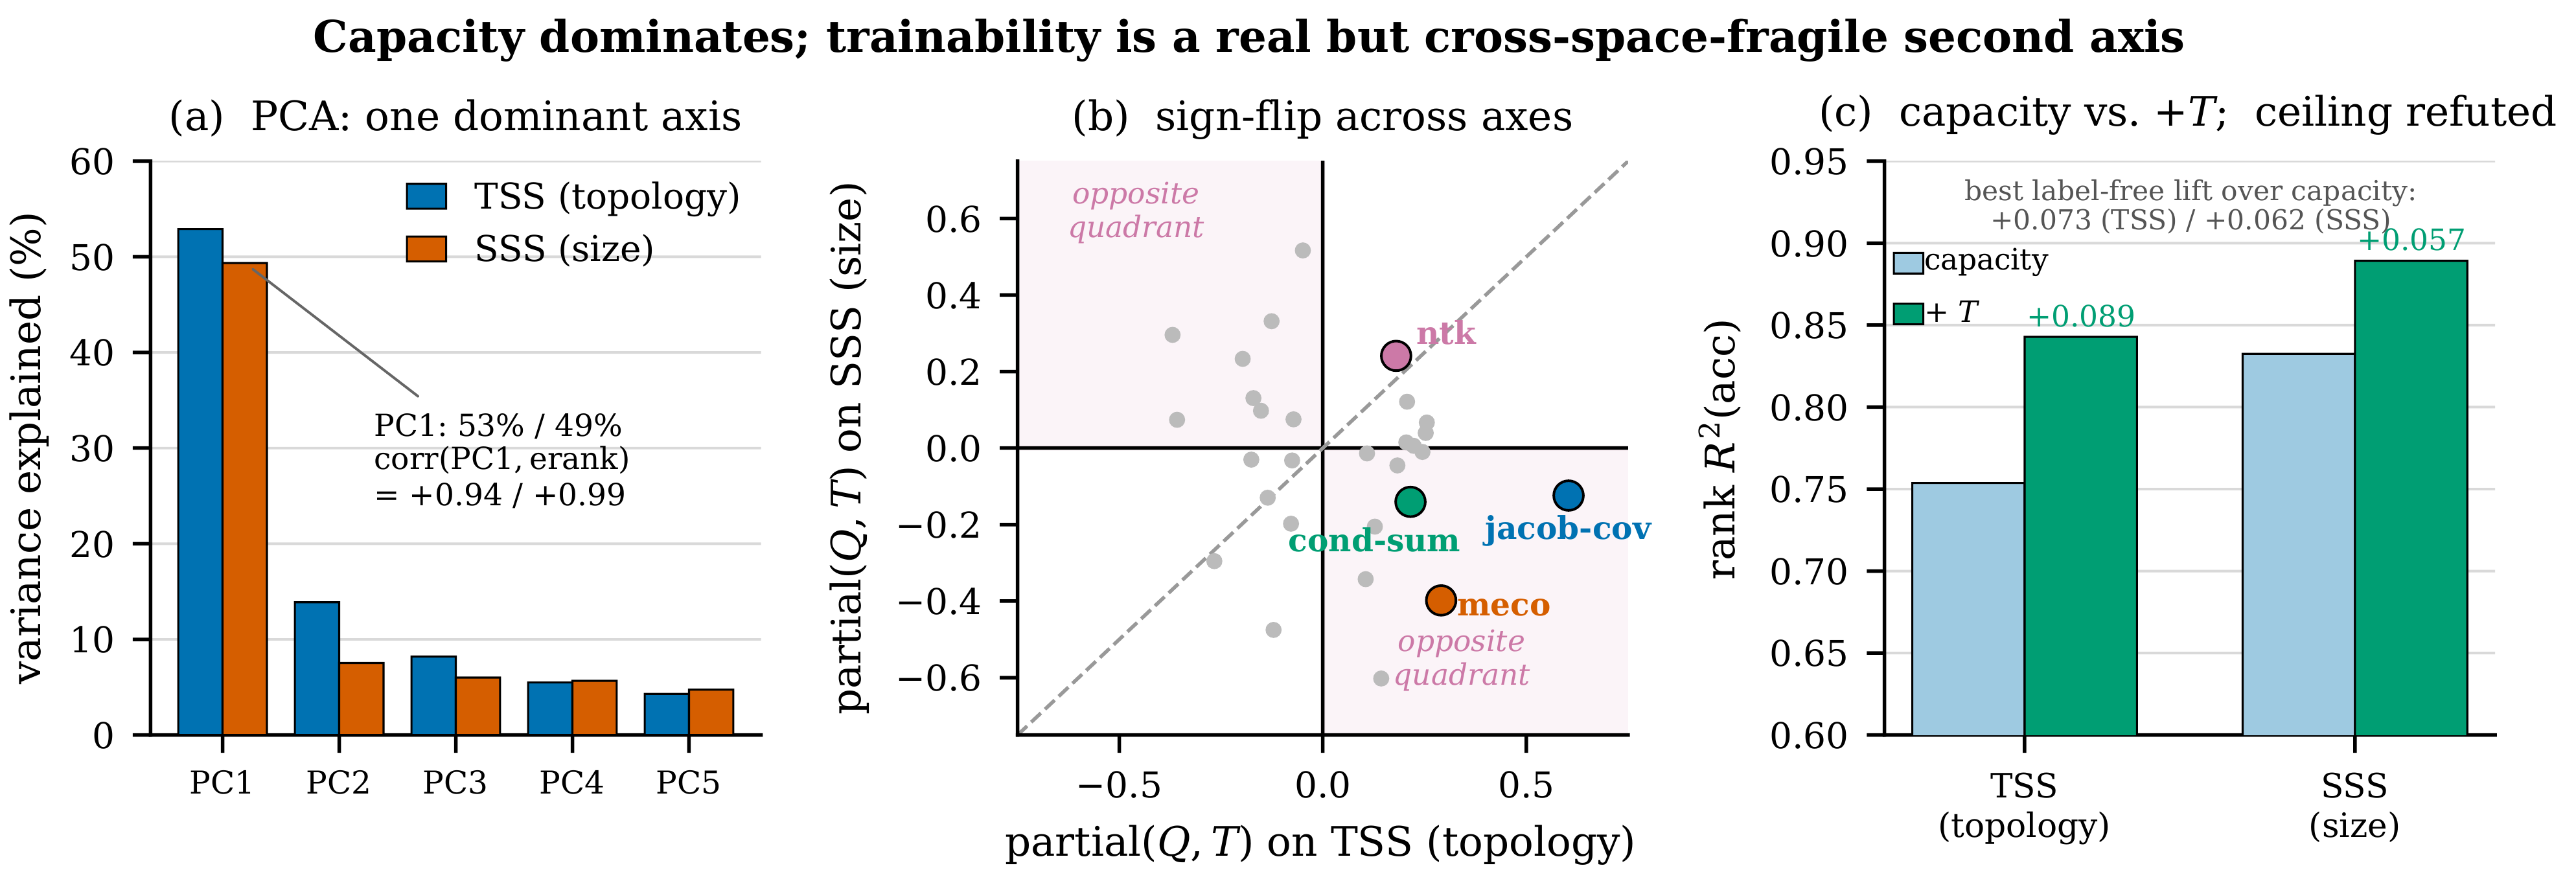
\includegraphics[width=\linewidth,trim=0 0 0 28.5bp,clip]{figures/fig3_results_final.png}
  \caption{\textbf{Capacity is dominant; the early-training association is
  cross-space-fragile.}
  \textbf{(a)} PCA scree of the oriented zoo, PC1 tracking effective rank;
  \textbf{(b)} per-proxy partial $\partialcorr(Q,T\mid\erank,\params)$ on TSS
  ($x$) vs SSS ($y$), opposite-sign quadrants shaded;
  \textbf{(c)} rank-$R^2(\acc)$ of capacity alone vs ${+}$ground-truth $T$ vs
  ${+}$axis-specific best label-free proxy (\px{meco}/\px{synflow}).}
  \label{fig:results}
\end{figure*}

%-------------------------------------------------------------------------
% RESULT 1 -- capacity dominance.
%-------------------------------------------------------------------------
\noindent\textbf{Capacity dominance (a confirmatory replication anchor).}\label{find:capacity}\label{sec:result1}\label{sec:r1}{}
To first order the proxies share a capacity-associated factor: the leading
component scores strongly track effective rank on both axes ($n{=}317/138$
complete cases). That component
carries about half the variance ($52.9\%$ TSS / $49.4\%$ SSS;
\cref{tab:cap-pc1}). Raw and globally fixed orientation leave these quantities
unchanged, but reduce the cross-axis loading cosine from $0.869$ to $0.461$;
thus the shared factor recurs, while its loading direction does not transport as
strongly as the per-axis outcome orientation suggested
(\cref{fig:results}a; Supplementary Sec.~\ref{app:r2-orientation},
\emph{Orientation control}). This reproduces the established
``proxies $\approx$ params/capacity'' reading of
\cite{ning2021evaluating,white2021powerful,kadlecova2024graf}, and serves as the
capacity-association anchor for the rest of the section rather than a co-equal headline. The
dominance is not an artifact of the R\'enyi sweep that supplies many oriented
proxies: a $12$-proxy rank-PCA with \emph{no} R\'enyi sweep still leaves a single
axis closely aligned with effective rank (\cref{tab:cap-pc1}). Exact PC1
correlations and the top-$14$ loadings are in \cref{app:pca-values}
(\cref{tab:app-pca}).

\noindent\textbf{Matched-sample-count control.}
Across 1,000 without-replacement TSS subsamples of $n{=}138$, PC1 variance stays
in $[0.497,0.559]$, its effective-rank association in $[0.918,0.953]$, and the
\px{cond-sum}, \px{meco}, and \px{grasp} reversals retain their direction in
every sample. These algorithmic summaries rule out simple sample-size imbalance,
not the separate SSS representativeness limitation (matched-$n$ intervals in
\cref{app:r2-sampling}).

%-------------------------------------------------------------------------
% RESULT 2 -- trainability is real.
%-------------------------------------------------------------------------
\noindent\textbf{A capacity-orthogonal trainability association remains.}\label{find:trainreal}\label{find:trainability}\label{sec:result2}{}
A nonzero, capacity-orthogonal \emph{trainability association} remains once capacity
is fixed: $\partialcorr(T,\acc\mid\erank,\params){\approx}{+}0.6$, replicating
across all three NB201 datasets. This term is what makes
the decomposition worth running, since if capacity were the whole story nothing
about trained accuracy would survive conditioning on it. The residual is carried
by the externally measured early-training descent rate $T$ (a benchmark
measurement, not a proxy self-check): adding ground-truth $T$ on top of capacity
raises rank-$R^2(\acc)$ from $0.7537$ to $0.8429$ on TSS ($95\%$ CI
$[0.798,0.880]$) and comparably on SSS, increments that clearly exceed a random
third predictor's noise floor (\cref{fig:results}c) and stay positive under
loss-based and slope-based $T$ (\cref{app:cvmethod}). Per dataset, parameters alone
explain about half the rank-$R^2$ while $T$ and effective rank each add a comparable
capacity-orthogonal share, the two together reaching $\sim\!0.83$ everywhere
(\cref{tab:decomp-body}; full grid \cref{tab:app-decomp}).

\begin{table}[t]
\centering\small\setlength{\tabcolsep}{4pt}
\begin{tabular}{lrrrr}
\toprule
& \multicolumn{4}{c}{leakage-clean rank-$R^2(\acc)$ ($R^2_{\mathrm{cv}}$)}\\
\cmidrule(lr){2-5}
Dataset & \px{params} & ${+}T$ & ${+}\erank$ & ${+}T{+}\erank$\\
\midrule
CIFAR-10      & $+0.526$ & $+0.775$ & $+0.730$ & $+0.828$\\
CIFAR-100     & $+0.541$ & $+0.743$ & $+0.778$ & $+0.840$\\
IN16-120      & $+0.482$ & $+0.777$ & $+0.727$ & $+0.837$\\
\bottomrule
\end{tabular}
\caption{\textbf{The descriptive pattern recurs across all three NB201 datasets:}
leakage-clean rank-$R^2(\acc)$ ($n{=}324$), where $T$ and $\erank$ each add a
comparable, capacity-orthogonal share on every dataset (\cref{find:trainreal}).}
\label{tab:decomp-body}
\end{table}

%-------------------------------------------------------------------------
% RESULT 3 -- partly accessible at init.
%-------------------------------------------------------------------------
\noindent\textbf{Some early-training signal is predictable at init.}\label{find:accessible}\label{find:access}\label{sec:result3}{}
This trainability residual is partly predictable from at-init statistics.
Regressing capacity $\{\erank,\params\}$ out of both accuracy and every proxy
\emph{inside each cross-validation train fold} (\cref{app:cvmethod}), the recovered
out-of-fold accuracy residual transfers to $T$ itself
($\partialcorr(\widehat{\mathrm{res}},T\mid\erank,\params){=}{+}0.536/{+}0.606$).
The key number is what \emph{survives} a strict leakage-clean test: the
all-proxy-over-best-single complementarity gain, ${+}0.2955$ (${+}103.2\%$, TSS) /
${+}0.0644$ (${+}17.7\%$, SSS).\footnote{The NBSZ-comparable pre-residual replicate
is the smaller ${+}13.8\%$ / ${+}1.0\%$; \cref{app:access-evidence}.} The held-out
associations are strongest for \px{jacob-cov} (${+}0.604$)
and the Jacobian/NTK family on topology, the gradient proxies on size, most proxies
not at all (\cref{app:access-evidence}, \cref{tab:app-perproxy}). The per-proxy
partial directions often differ under per-axis outcome-informed orientation
(\cref{fig:results}b), whose sensitivity is resolved in \cref{sec:crossspace}.

%-------------------------------------------------------------------------
% RESULT 4 -- no binding ceiling (self-refutation); folds in frozen-NTK test.
%-------------------------------------------------------------------------
\noindent\textbf{No empirical label-free ceiling on these benchmarks.}%
\label{find:noceiling}\label{find:ceiling}\label{sec:result5}{}
The first three results invite a reading in which the rest of accuracy is a hard
limit only training breaks, Proposition~\ref{thm:bound}'s ceiling reading
transposed onto trained accuracy. The data do not support that reading on these
benchmarks. Over capacity $\{\erank,\params\}$, \px{meco} on TSS and \px{synflow}
on SSS already lift rank-$R^2(\acc)$ by ${+}0.0728$ / ${+}0.0616$, while the additional gap
closed \emph{only} by substituting ground-truth $T$ is just ${+}0.0164$ (TSS) /
${-}0.0048$ (SSS) (\cref{fig:results}c), too small to be a ceiling.

\noindent\textbf{The direct NTK test preserves the proposition's narrow scope.}
On 324 TSS architectures, the frozen at-init NTK error correlates only
$\rho{=}0.40$ $[0.29,0.49]$ with trained accuracy, although a finite 30-feature
dictionary predicts both well. Proposition~\ref{thm:bound} therefore prices that
frozen-kernel target, not trained accuracy; full family and ridge results are in
\cref{app:ntk}.

\smallskip
\noindent
For the evaluated examples, an early-training association is accessible at init,
but its direction is less portable than its within-axis magnitude; this motivates
the transport analysis in \cref{sec:crossspace}.

\section{What Flips: The Cross-Space Sign Reversal}
\label{sec:crossspace}

%% ---------------------------------------------------------------
%% Cluster: the sign-flip and its consequences. The page-1 concept
%% figure (\cref{fig:signflip}) is defined in sec_v3/0_abstract.tex;
%% the hero exhibit of THIS cluster is the full-width portability
%% heatmap fig:portability, floated at the top.
%% ---------------------------------------------------------------

\begin{findingframe}
\textbf{The portability failure, in brief} (\cref{fig:portability}). A single
zero-cost proxy reverses the sign of its relationship to quality when moved
between two axes of the same benchmark. Three within-NB201 examples motivate the
analysis; $9/13$ proxies reverse descriptively somewhere in the broader map and
four cross-benchmark cases meet the strict support rule. The \px{cond-sum}
failure is dimension-linked, and two named budget-search traps cost $+5.40$ and
$+1.97$ accuracy points at $K{=}10$, while two null directions cost zero.
\end{findingframe}

\noindent We summarize above and elaborate next.

%-------------------------------------------------------------------------
% HERO EXHIBIT: 13x7 cross-space portability heatmap (full-width figure*).
%-------------------------------------------------------------------------
\begin{figure*}[t]
  \centering
  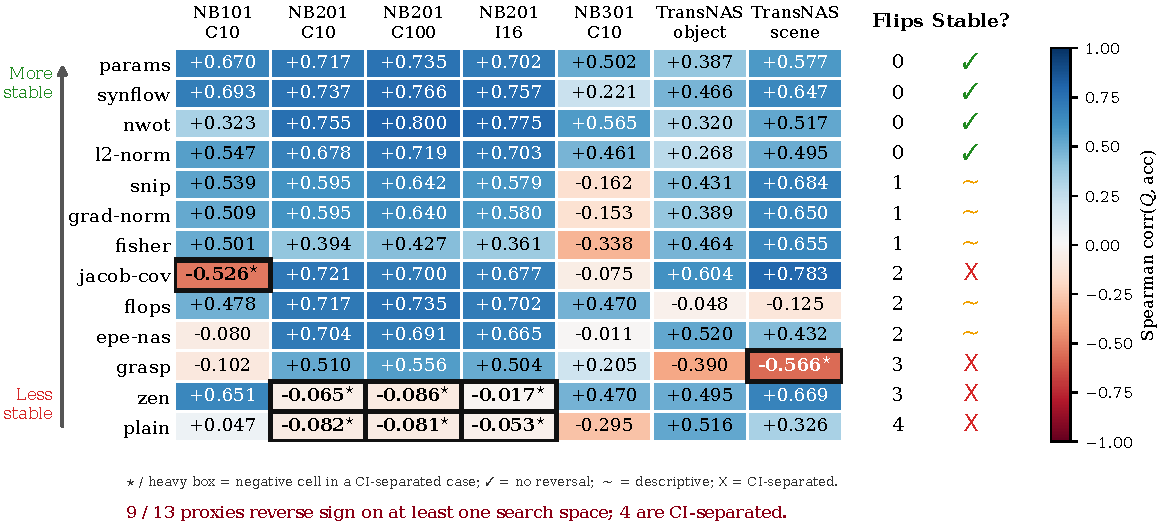
\includegraphics[width=\textwidth]{figures/fig4_portability_full.pdf}
  \caption{\textbf{Cross-space portability matrix.} Spearman
  $\corr(Q,\acc)$ for $13$ standard proxies over $7$ search spaces, with rows
  ordered most-to-least stable (flip count ascending, then mean $|\rho|$).
  Heavy boxes and $\star$ mark negative cells in the four CI-separated cases
  (\px{jacob-cov}, \px{grasp}, \px{zen}, \px{plain}); the side panel reports
  each proxy's flip count and stability tier ($\checkmark$: no reversal;
  $\sim$: descriptive reversal; $\mathsf{X}$: CI-separated reversal). Nine of $13$ proxies
  reverse descriptively on at least one space, while four meet the strict rule.
  Per-space sample sizes and intervals are in \cref{tab:app-portability} and
  \cref{app:generalize-evidence}.}
  \label{fig:portability}
\end{figure*}

\noindent\textbf{The cleanest instance lives \emph{inside} a single benchmark.}
The preceding analysis (\cref{sec:cap-train}) found a capacity-associated factor
that recurs on both axes
and a trainability residual that is statistically distinct and partly accessible. We
now ask whether a single proxy carries the same signal once it is moved to a
structurally different axis. NB201's two one-knob axes (\cref{sec:setup}) let a
reversal be read off without blaming a change of dataset, recipe, or proxy
implementation. We therefore center the orientation-free accuracy correlation
$\corr(Q,\acc)$ and treat the per-proxy trainability partial
$\partialcorr(Q,T\mid\erank,\params)$ as an orientation-sensitive secondary view.

%-------------------------------------------------------------------------
\noindent\textbf{The sign-flip.}\label{sec:result4}\label{sec:r4}\label{sec:signflip}\label{find:flip}{}
The cleanest, orientation-free result is the raw accuracy-slot flip: a single
proxy's correlation with quality reverses from positive on the topology
(TSS) axis of NAS-Bench-201 to negative on the size (SSS) axis, with no
sign-orientation rule applied. The spectral conditioning functionals make this
plain: \px{cond-sum} goes $+0.88\,{\to}\,-0.77$ ($n{=}324/138$),
\px{meco} $+0.88\,{\to}\,-0.79$, and \px{grasp} $+0.55\,{\to}\,-0.19$, the page-1
headline (\cref{fig:signflip}). The spectral arm also clears a faithfulness
check: the TSS value is consistent with Dextr's published $\sim\!0.88$
(\px{cond-sum} = the official inverse-condition statistic, $0$ hook exceptions;
\cref{app:faithfulness}), making a simple TSS implementation mismatch less
plausible. A
reversal this large in the raw, un-oriented accuracy slot is the central flip we
analyze.

\noindent Under per-axis outcome-informed orientation, the same reversal also reaches the trainability partial
$\partialcorr(Q,T\mid\erank,\params)$, the very slot previewed in
\cref{fig:results}(b), though here the evidence is more graded. The CI-separated
trainability-slot reversals across both axes are carried by \px{meco}
($+0.291\,{\to}\,-0.398$) and \px{Q-adapt-rot} ($+0.143\,{\to}\,-0.602$); the
headline \px{cond-sum} SSS trainability partial is $-0.141$ with $95\%$ CI
$[-0.31,+0.04]$, which spans zero, so it is consistent-with rather than a
CI-separated trainability-slot flip, as are the SSS partials for \px{jacob-cov}
and \px{gradsign} (\cref{app:perproxy-signflip}, \cref{tab:app-perproxy}).\linebreak One
caveat is decisive: because each proxy was sign-oriented per axis by its own
accuracy correlation, the trainability-slot direction is entangled with the
outcome-informed rule. In the global-orientation control, PCA variance and
score/capacity association are unchanged but loading agreement drops from
$0.869$ to $0.461$; \px{meco}'s SSS partial also changes orientation. We therefore
treat these trainability-slot directions as orientation-sensitive exploratory
evidence, not as an independent cross-axis flip. The raw accuracy-slot reversals
above remain orientation-free.

%-------------------------------------------------------------------------
\noindent\textbf{The outcome-informed orientation's narrow survivor.}\label{sec:mechanism}\label{find:ntk}\label{find:mech}{}
Under per-axis outcome-informed orientation, one proxy---\px{ntk}---has a \emph{trainability partial}
$\partialcorr(Q,T\mid\erank,\params)$ that is positive with a CI excluding zero on
both axes ($+0.180$ TSS / $+0.241$ SSS); its $T_{\mathrm{slope}}$ partial also
survives BH-FDR on both axes. The qualifier matters: \px{ntk} survives
\emph{in this trainability-partial slot at the full-zoo sample}, not as a portable
accuracy predictor---as a raw accuracy ranker it is anti-correlated on \emph{both}
axes (\cref{tab:app-perproxy}). This is not an orientation-robust uniqueness
claim: under the globally fixed rule both \px{meco} and \px{ntk} have positive
marginal intervals on both axes, an exploratory, unadjusted comparison. At the
larger standard-proxy base \px{synflow} and \px{zico} also join \px{ntk} under
this rule; per-proxy cells are in \cref{app:mechanism-evidence}.

\noindent\textbf{The \px{cond-sum} failure is dimension-linked, not an identified
mechanism.} On balanced $n{=}500/500$ cohorts, the raw correlation is
$+0.887/-0.781$ (TSS/SSS). Dividing by cached spectrum length gives
$+0.842/-0.785$, and dividing by effective rank gives $+0.418/-0.885$.
Within SSS, however, the partial of the raw score is only $-0.079$ after
effective-rank control and $-0.068$ after joint cached-length, effective-rank,
and parameter controls. Exact cached-length matching is not identifiable because
the supports do not overlap (TSS $142$--$502$; SSS $118$--$122$). An unmatched
effective-rank common-range sensitivity yields $-0.318/-0.885$, removing the
cross-axis sign difference, but only 103 TSS records fall in that range. Finally,
the cached count is not a validated representation dimension. These results
support a dimension-linked/proxy-geometry-dependent transport failure. An exact
representation-dimension-matched test cannot be performed because that field is
absent from the available artifacts.

%-------------------------------------------------------------------------
\begin{table}[H]
\centering\small\setlength{\tabcolsep}{5pt}
\begin{tabular}{lrr}
\toprule
Score correlation ($n{=}500$ per axis) & TSS & SSS\\
\midrule
\px{cond-sum} (raw) & $+0.887$ & $\mathbf{-0.781}$\\
\px{cond-sum}/cached length & $+0.842$ & $\mathbf{-0.785}$\\
\px{cond-sum}/effective rank & $+0.418$ & $\mathbf{-0.885}$\\
$R_{\alpha=1}$ (effective rank, NEAR) & $+0.864$ & $+0.911$\\
\bottomrule
\end{tabular}
\caption{\textbf{Cached normalizations do not by themselves remove the
full-population flip.} Effective-rank partial/common-range sensitivities and the
non-overlapping cached-length support require the narrower dimension-linked
interpretation in the text.}
\label{tab:spectral-body}
\end{table}

\noindent Full normalization intervals, within-length strata, the common-range
sensitivity, and the reason exact dimension matching is unavailable are in
\cref{app:r2-dimension}.

\noindent\textbf{It partly generalizes.}\label{sec:generalize}\label{find:generalize}{}
Of the $9$ proxies that reverse the sign of $\corr(Q,\acc)$ on at least one of the
seven columns, exactly four survive a strict test---two columns whose
$2000$-resample $95\%$ intervals are disjoint, each individually FDR-significant---and
they fall into two magnitude tiers (\cref{fig:portability}). Two are large
bilateral flips: \px{jacob-cov} ($+0.78$ TransNAS-scene vs.\ $-0.53$ NB101) and
\px{grasp} ($+0.56$ NB201-CIFAR-100 vs.\ $-0.57$ TransNAS-scene). The other two are
attenuations-to-near-zero rather than full reversals: \px{zen} ($+0.67$ vs.\
$-0.086$) and \px{plain} ($+0.33$ vs.\ $-0.082$), whose negative side is significant
only by the large NB201 sample. The remaining candidates fail the bar---small-$n$
NB301 attenuations, \px{epe-nas}'s lone NB101 cell, and \px{flops}'s near-zero TransNAS
reversal---and only NB301 stays excluded as degenerate
(\cref{app:generalize-evidence}). This cross-space arm reintroduces the dataset and
sample-size confounds the within-NB201 design removed, so these four flips are
weaker evidence than the within-benchmark reversal. The decomposition behind this
also replicates across NB201's three datasets---capacity stays the leading term and
trainability a comparable contributor (\cref{tab:decomp-body})---while the deep
capacity/trainability decomposition itself remains NB201-only. Full per-space
values and CIs are in \cref{app:generalize-evidence},
\cref{tab:app-portability,tab:app-spectral}, and \cref{app:crossspace}.

\noindent\textbf{Recent controls bound the claim.}
SWAP~\cite{peng2024swap} is positive on TSS/SSS ($0.798/0.778$), as is
AZ-NAS~\cite{aznas2024} ($0.922/0.740$),
with architecture-bootstrap intervals excluding zero. Thus SWAP is one
sign-stable recent control, not evidence about every recent proxy;
L-SWAG~\cite{casarin2025lswag}/InTrain~\cite{intrain2026}
remain unevaluated because no official, licensed, auditable implementation was
available as of August 25, 2026 (intervals and protocol in
\cref{app:r2-recent}).

\noindent\textbf{The full decomposition remains NB201-only.}
Across 49,674 audited external records, official artifacts expose only 13 finite
proxy fields and lack the complete aligned proxy/capacity/training field classes
required by \cref{eq:decomp}. No population jointly has sufficient proxy
coverage, effective rank, exact early $T$, and final accuracy, so
\cref{eq:decomp} has zero eligible external rows. We report the missing-field
coverage instead of constructing a surrogate, while retaining the raw map beyond
NB201 (audit in \cref{app:r2-external}).

%-------------------------------------------------------------------------
\noindent\textbf{The flip has a search cost.}\label{sec:searchtransfer}\label{find:searchtransfer}{}
The reversal changes which architecture a budget-$K$ search returns. The baseline
transfers the single best-on-source proxy as-is; the sign-stability screen uses a
target-CALIB split to reject a proxy whose orientation does not transport, then
scores a disjoint target-EVAL split. No network is trained, but cached target
accuracy is used for calibration. On the TSS${\to}$SSS trap, the gap to
the source-best proxy is $+7.83/+6.62/+5.40/+3.00$ at $K{=}1/5/10/50$.
The scene${\to}$NB101 trap gives $+1.11/+1.55/+1.97/+1.56$; the reverse
SSS${\to}$TSS and scene${\to}$NB201 nulls are zero at every budget. At the
pre-specified moderate budget $K{=}10$, percentile intervals under the
target-position resampling protocol are
$[4.386,6.435]$ and $[0.626,3.133]$ for the two traps
(\cref{tab:searchtransfer}). All $K{=}1/5/10/50$ results are retained to avoid
favorable-budget selection. These are named trap costs, not average gains.

%-------------------------------------------------------------------------
\noindent\textbf{The diagnostic is target-calibrated, not fully label-free.}{}
The CALIB and EVAL positions are disjoint under the target-position
resampling protocol, but
canonical architecture identities can overlap. A second protocol partitions
identities first and has zero CALIB/EVAL identity overlap; its K=10 intervals are
$[5.057,5.599]$ and $[1.487,2.208]$, with both nulls still zero. The protocols
use different resampling units and are reported separately. The evaluation
also includes params, SynFlow, fixed rank-ensemble, random, negative, and
unfavorable comparisons. The screen is useful for the two evaluated trap
directions, but
does not dominate every baseline and is not a universal NAS remedy.
Full budget results, baseline comparisons, and the identity-disjoint sensitivity
are reported in Supplementary Sec.~\ref{app:r2-search}
(\emph{Search consequence and sensitivity protocols}).

\begin{table}[htbp]
  \centering
  \small
  \caption{\textbf{K=10 search consequence} (cached accuracy, no training).
  Values are target-CALIB screen minus transported source-best proxy; intervals
  are non-inferential percentile summaries under the target-position
  resampling protocol.}
  \label{tab:searchtransfer}
  \begin{tabular}{@{}lrc@{}}
    \toprule
    Direction & gap (pts) & percentile interval \\
    \midrule
    TSS${\to}$SSS (trap) & $+5.402$ & $[4.386,6.435]$ \\
    SSS${\to}$TSS (null) & $0.00$ & $[0,0]$ \\
    scene${\to}$NB101 (trap) & $+1.973$ & $[0.626,3.133]$ \\
    scene${\to}$NB201 (null) & $0.00$ & $[0,0]$ \\
    \bottomrule
  \end{tabular}
\end{table}

\paragraph{Multiple-comparison control.}
The strict cases do not rely only on unadjusted screening: $34$ of the $58$
per-proxy partial cells and $78$ of the $91$ portability cells survive BH-FDR,
and each of the four CI-separated
flips is individually FDR-significant; the full accounting is in \cref{tab:app-fdr}
(\cref{app:generalize-evidence}).

%-------------------------------------------------------------------------
% The released artifact, as the closing subsection of "What Flips" (sec:crossspace).
% Full datasheet/datacard + the population-reconciliation table live in
% \cref{app:datasheet} (App I) so this body unit stays compact.
%-------------------------------------------------------------------------

\subsection{A reusable cross-space portability map}
\label{sec:artifact}
We construct a $13{\times}7$ cross-space portability map
(\cref{fig:portability}, \cref{tab:app-portability}) from per-architecture proxy
values and per-(proxy, space-pair) \emph{sign-stability flags}. These full-data
flags are retrospective descriptive annotations, not inputs to the evaluated
screen. In the search experiment of \cref{find:searchtransfer}, the target sign
is re-estimated separately within each split from target-CALIB cached accuracy,
without using target-EVAL. A population-reconciliation table
(\cref{tab:reconcile}) and the full datasheet (schema, splits,
intended use, limitations; \cref{app:datasheet}) accompany it; the map will be released under a permissive open-source license, with
a permanently archived and citable snapshot, upon publication.

%-------------------------------------------------------------------------
% NOTE: The page-1 concept figure (\cref{fig:signflip}), the multi-panel
% results figure (\cref{fig:results}), the portability heatmap
% (\cref{fig:portability}), and Proposition 1 (\cref{thm:bound}) are defined
% in earlier sections. This section only \cref's them.
%-------------------------------------------------------------------------

\section{Conclusion and Limitations}
\label{sec:discussion}

\textbf{What travels, and what flips.}
\label{sec:disc-refute}\label{sec:disc-measure}\label{sec:disc-cross}\label{sec:disc-org}\label{sec:conclusion}%
The diagnostic picture is mixed. A dominant capacity-associated factor recurs
on both axes: its variance share and score/effective-rank association recur,
although its loading direction is outcome-orientation-sensitive
(\cref{find:capacity}). Raw proxy/accuracy relations can \emph{flip} (e.g.\
\px{cond-sum} $+0.88\,{\to}\,-0.77$; \cref{fig:signflip}). A
capacity-orthogonal early-trainability association remains partly accessible at
initialization, although its per-proxy directions are also orientation-sensitive
(\cref{find:trainreal,find:accessible}). Thus \px{cond-sum} indicates a
dimension-linked/proxy-geometry-dependent transport failure, not an identified
mechanism. Our data also do not support a ``label-free ceiling'': \px{meco} on
TSS and \px{synflow} on SSS recover much of the trainability gap
(\cref{fig:results}c; \cref{find:noceiling}). Proposition~\ref{thm:bound}
certifies only a squared-correlation bound for a \emph{frozen at-init NTK}
target, not trained accuracy.

\textbf{The practical rule.}
Validate a zero-cost proxy's orientation on the target axis before transporting
its source ranking. In two named traps, a target-CALIB screen avoids $+5.40$ and
$+1.97$ point costs at $K{=}10$; two null directions remain unchanged
(\cref{find:searchtransfer}). The diagnostic uses cached calibration labels,
does not dominate every baseline, and is not a fully label-free or universal
remedy.

\textbf{Limitations.}
\label{sec:limitations}%
All results are observational benchmark correlations. Matched-$n$ resampling
addresses sample count, but SSS representativeness and true dimension matching
remain unresolved. External flips reintroduce dataset/$n$ confounds; the
decomposition is NB201-only, and unconstrained deployment plus
optimizer/initialization/regime interventions remain future work.


{\small
\bibliographystyle{ieeenat_fullname}
\bibliography{main}
}

\end{document}
